\documentclass[10pt]{beamer}
\usepackage{verbatim}
\usepackage{amsmath}
\usepackage{amsthm}
\usepackage{graphics}
\usepackage{color}
\usepackage{stmaryrd}\usefonttheme[onlymath]{serif}

\title{Discussion 2}
\date{\today}

\begin{document}
\maketitle


\begin{frame}\frametitle{Crucial Problem}
Different from the disjunctive invariant problem, which only needs to generate a max-plus convex to surround the samples, the dependcy relation between different parts is much more important in multiphase ranking function.

So the crucial problem is to find a effective way to split these area.

\end{frame}


\begin{frame}\frametitle{Idea1: Blocks}
Use disjunctive terms of the loop guards and branch guard for multiphase ranking function.
\begin{center}
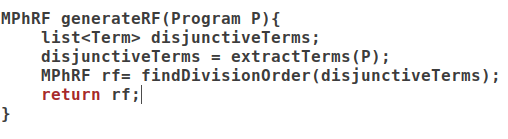
\includegraphics[scale=0.5]{2.png}
\end{center}
\end{frame}

\begin{frame}\frametitle{Immature Idea2}
Consider the space of the program states. Given a transition between two states, we got a vector $\vec{x} = \textbf{x'} - \textbf{x}$. Now given two vectors, $\vec{x}, \vec{y}$ where they are both possible transition of the loop. If they are in the same region, then we require they are both ranked by the same ranking function. Assume  the normal vector of ranking function $f(\textbf{x}) = \vec{a}\textbf{x} + b$ is $\vec{n}$. Then in this region $\vec{x}\cdot\vec{n} \times \vec{y}\cdot\vec{n} > 0$. 

Can we use sampling methods for splitting the ranked area? i.e. use the condition above the find a splitting hyperplane in the transition space.





\end{frame}


\begin{frame}
\begin{center}
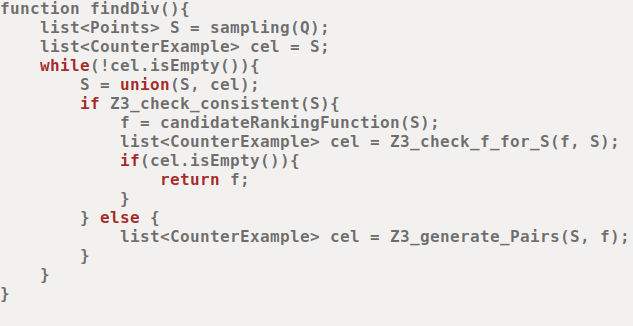
\includegraphics[scale=0.5]{1.png}
\end{center}
\end{frame}


\begin{frame}\frametitle{Irrelevant Idea3}
Question: Is a partial ranking function useful? Here partial means only a part of the transitions of the loop are ranked but not all. Can we use this information to shrink the space we consider for generating counterexample for nontermination?



\end{frame}

\begin{frame}\frametitle{Idea4: Use Max- and Min-Plus for Multiphase RF}
Definition of Max-Plus:
\[\max(c_1, c_2 + x_2, \ldots, c_n + v_n) \ge \max(d_1, d_2 + x_2, \ldots, d_n + x_n)\]

If we use $f_i(x)$ to replace original $x_i$, maybe we cannot utilize some feature or algorithms.

Try: consider a 2-phase ranking funtion

\[f_1(x) \ge 0 \wedge \Delta f_1(x'') \ge 1 \vee\]
\[ f_1(x) < 0 
\wedge \Delta f_1(x'') \ge 1 \wedge f_2(x) \ge 0 \wedge \Delta f_2(x'') \ge 1\]


\[a \ge 0 \wedge b \ge 0 \vee\]
\[a  < 0 \wedge b \ge 0 \wedge c \ge 0 \]


\end{frame}

\begin{frame}

\[a \ge 0 \wedge b \ge 0 \vee\]
\[a  < 0 \wedge b \ge 0 \wedge c \ge 0 \]

is equivalent to:
\[a \ge 0 \wedge b \ge 1 \wedge c \ge 0  \vee\]
\[a \ge 0 \wedge b \ge 1 \wedge c < 0  \vee\]
\[a  < 0 \wedge b \ge 1 \wedge c \ge 0 \wedge d \ge 1\]
If ignore $d \ge 1 $ we have
\[\max(a, c) \ge 0 \wedge b\ge 1\]
If not 


\[\max(a, c) \ge 0 \wedge b\ge 1 \wedge (a < 0 \wedge c \ge 0 \rightarrow d \ge 1 )\]
\[\max(a,c)\ge 0 \wedge b \ge 1 \wedge (a \ge 0 \vee c < 0 \vee d \ge 1 )\]
\[\max(a,c)\ge 0 \wedge b \ge 1 \wedge ( c < 0 \vee \max(a, d-1)\ge 0)\]
\[\max(a,c)\ge 0 \wedge b \ge 1 \wedge  \max(-c, \max(a, d-1))\ge 0\]
\end{frame}


\end{document}